\documentclass[12pt]{article}
\usepackage{amsmath, amsfonts}
\usepackage{graphicx}
\usepackage{tabularx}

\graphicspath{{./img}}
\usepackage[margin=1in]{geometry}

\usepackage{xeCJK}
\setCJKmainfont{WenQuanYi Micro Hei Mono}

\usepackage{algorithm}

\usepackage[backend=biber,style=ieee]{biblatex}
\addbibresource{report.bib}

\begin{document}
\title{Data Science Homework 4}
\author{Andr\'es Ponce,
\and
彭思安
\and
P76107116
}

\begin{document}
\maketitle
\section{Introduction}
Our data's properties will determine the pre-processing steps we take to ensure our 
model performs well with new data.
For instance, since machine learning methods can for the most part deal only with
numerical values, its is necessary to convert string-based values into numbers.
Such methods range from just assigning a numerical value to a class index to 
using hash tables to store indices of the column to which it belongs.

Another common issue in the data processing stage is imbalanced data.
This happens when some categories in our data happen less often than others,
sometimes much less often.
These categories are known as \textbf{minority class}, and more common
classes or categories are known as \textbf{majority class}.
To ensure our model is exposed to the category, we can either remove elements
from the majority class with \textbf{undersampling methods} or create new samples
from the minority class using \textbf{oversampling methods}.

In this assignment we investigate the relation between datasets and different
encoding and sampling methods.
First, we describe the datasets used, then conduct experiments on different
combinations of encoding and sampling methods.

\section{Datasets}
% Make the table here
% Plot the class imbalances
\begin{centering}
\begin{table}
\begin{tabular}{|c|c|c|c|c|c|}
	\hline
	Dataset & Features & Categorical & Numerical & Size & Task \\
	\hline
	Heart Disease & 14 &  11 & 3 & 319,795 &  Multi-class \\
	\hline
	Bank Marketing & 20 & 9 & 11 & 32561 & Binary \\
	\hline
	Income Evalutaion & 15 & 9 & 6 & 32,562 & Binary \\
	\hline
	Telco Customers & 21 & 19 & 2 & 7044 &  Binary \\	
	\hline
	Abalone & 8 & 1 & 8 & 4178 & Multi-Class \\
	\hline
	IBM Attrition & 13 & 4 & 9 & 1470 & Multi-Class \\
	\hline
	Biostar Degradation &42&0&42&1055&Binary \\
	\hline
	ECommerce & 11 & 4 &  7 & 11,000 & Binary\\
	\hline
	Fuel Consumption & 15 & 9 & 6 & 947 & Multi-Class \\
	\hline
	Travel Insurance & 10 & 4 & 6 & 1986 & Binary \\
	\hline
	Diabetes & 15 & 1 & 14 & 520 & Binary \\
	\hline
	Loans & 10 & 5 & 5 & 399 & Binary \\
	\hline
	Onlne Shopper intention & 18 & 8 & 10&  12,330 & Binary \\
	\hline
	Teacher Assistant & 6 & 5 & 1 &  150 & Multiclass \\
	\hline
	Churn Modelling & 14 & 2 & 12 & 10,000 & Binary \\
	\hline
	\label{table:datasets}
\end{tabular}
\caption{Properties of the datasets used.}
\end{table}
\end{centering}

\
In this assignment, we used 15 classification datasets, most of which have a class imbalance.
The datasets were mostly obtained mostly from Kaggle, the UCI repository, and OpenML.
Table~\ref{table:datasets} shows basic information about our datasets.
Some of the tasks involve doing binary classification, where the target class has only two 
distinct values, while others have multiple target values.
Imbalanced datasets are often handled using measures such as \textbf{precision}
and \textbf{recall}, which measure the percentage of correct classifications and 
and the percentage of samples we correctly classified as belonging to a different 
class, respectively.

With multiclass datasets, we can take each class $c_i$ as the positive 
class and all the other classes as the negatives.
The \texttt{imblearn} library provides functions to calculate the precision, 
recall, F score, and support for each class.

\begin{figure}
	\centering
	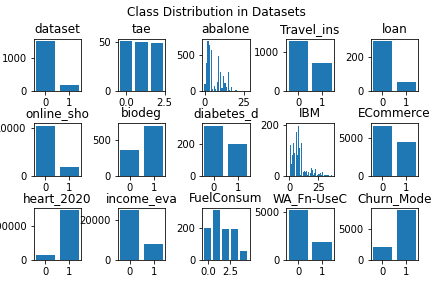
\includegraphics[scale=0.8]{distribution}
	\label{fig:dists}
	\caption{Distribution of the target labels of each file tested.}
\end{figure}

\section{How does feature scaling (i.e. doing standardization) affect the performance?}
To test the effect of standardization on the model performance, we train a \texttt{RandomForest}
classifier with 10 decision trees.
Since we want to measure the effect of standardization on performance
as a whole, we use classification accuracy as our measure.


\begin{table}
\begin{centering}
	\begin{tabular}{|c|c|c|}
	Dataset & Scaled & Non-Scaled \\
	\hline
	Heart Disease & 87.9 & 87.9 \\
	\hline
	Bank Marketing & 88.6 & 87.8 \\
	\hline
	Income Evaluation & 84.8 & 85.1 \\
	\hline
	Telco Customers & 78.3 & 78.8 \\
	\hline
	Abalone & 23.3 & 23.3\\
	\hline
	IBM Attrition & 15.9 & 14.2 \\
	\hline
	Biostar Degradation & 86.6 & 85.5 \\
	\hline
	Credit Card  & 66.2 & 66.6 \\
	\hline
	Fuel Consumption & 80 & 76 \\
	\hline
	Travel Insurance  & 80.6 & 80.7 \\
	\hline
	Diabetes  & 98.4 & 97.6 \\
	\hline
	Loans & 81.2 & 82.0 \\
	\hline
	Onlne Shopper intention & 89.6 & 89.4 \\
	\hline
	Teacher Assistant & 61.3 & 62 \\
	\hline
	Churn Modelling & 85.0 & 84.8\\
	\hline
	\end{tabular}
	\caption{Effects of applying feature standardizaiton.} 
	\label{table:scaling}
\end{centering}
\end{table}

As seen in Table~\ref{table:scaling}, in our experiments feature scaling 
has only a small influence in our accuracy. 
Some datasets such as IBM Attrition and Abalone had poor performance
because there are classes that have only one sample. 
This poses problems when using a \texttt{StratifiedKFold} cross-validation
method.
It is important that we use this evalutation method so we can roughly 
preserve the original distribution of data in each fold.
Most results fall within one percentage point difference between the
standardized and non-standardized approaches.

\section{When using tree-based algorithms, will using one-hot encoding for 
categorical features generate worse performance than label encoding? Why?}
Using one-hot encoding for a RandomForest classifier does indead lead to
worse performance, sometimes by significant amounts.
We run our experiments again using a \texttt{RandomForest} classifier
with 10 decision trees.

One-hot algorithms greatly increase the amount of columns in the dataset.
Tree-based classifiers using an impurity metric such as GINI have a greater
chance of using the new columns in their splits at every stage.
This means that we can end with deep decision trees that rely on these columns.

\begin{table}
\begin{centering}
	\begin{tabular}{|c|c|c|}
	\hline
	Dataset & One-Hot Encoding & Label Encoding \\
	\hline
	Heart Disease & & \\
	\hline
	Bank Marketing & 86.0 & 87.9 \\
	\hline
	Income Evaluation & & \\
	\hline
	Telco Customers & & \\
	\hline
	Abalone & & \\
	\hline
	IBM Attrition & & \\
	\hline
	Biostar Degradation & 81.6 & 86.0 \\
	\hline
	ECommerce & 65.7 & 66.1 \\
	\hline
	Fuel Consumption & 56.7 & 78.3 \\
	\hline
	Travel Insurance  & 74.5 & 80.2 \\
	\hline
	Diabetes  & & \\
	\hline
	Loans & & \\
	\hline
	Onlne Shopper intention & & \\
	\hline
	Teacher Assistant & & \\
	\hline
	Churn Modelling & & \\
	\hline
	\end{tabular}
	\caption{Effects of applying feature standardizaiton.} 
	\label{table:encoding}
\end{centering}
\end{table}

Table~\ref{table:encoding} shows the results of our encoding experiments.

\end{document}
